\documentclass[12pt,a4paper]{article}

% 导入必要的宏包
\usepackage[UTF8]{ctex}
\usepackage{geometry}
\usepackage{amsmath}
\usepackage{amsfonts}
\usepackage{amssymb}
\usepackage{graphicx}
\usepackage{enumitem}
\usepackage{xcolor}
\usepackage{tikz}
\usepackage{float}
\usepackage{hyperref}
\usepackage{multicol}
\usepackage{longtable}
\usepackage{array}
\usepackage{tabularx}

% 页面设置
\geometry{left=2.5cm,right=2.5cm,top=2.5cm,bottom=2.5cm}

% 标题页设置
\title{\textbf{2013年数据结构题库} \\ \large }
\author{}
\date{}

% 定义题型环境
\newenvironment{choicequestion}[1][]{%
    \vspace{0.5cm}
    \noindent\textbf{[#1]}
    \vspace{0.2cm}
}{}

\newenvironment{answersection}{%
    \vspace{0.2cm}
    \noindent\textbf{[参考答案]}\\
    \vspace{0.1cm}
}{}

\newenvironment{analysissection}{%
    \vspace{0.2cm}
    \noindent\textbf{[答案解析]}\\
    \vspace{0.1cm}
}{}

% 定义题号计数器
\newcounter{questioncounter}

% 问题格式化命令
\newcommand{\question}[2]{%
    \stepcounter{questioncounter}%
    \noindent\textbf{\thequestioncounter} #1%
}

% 选择题选项格式
\newcommand{\choices}[4]{%
    \begin{multicols}{2}
    \noindent \textbf{A.} #1 \par
    \noindent \textbf{B.} #2 \par
    \noindent \textbf{C.} #3 \par
    \noindent \textbf{D.} #4 \par
    \end{multicols}%
}

% 表格格式
\newcolumntype{Y}{>{\centering\arraybackslash}X}

% 开始文档
\begin{document}

\maketitle

\section{单项选择题}

\begin{choicequestion}[单选题]
\question{已知两个长度分别为 $m$ 和 $n$ 的升序链表，若将它们合并为一个长度为 $m + n$ 的降序链表，则最坏情况下的时间复杂度是}{D}
\choices{$\mathrm{O}(n)$}{$\mathrm{O}(mn)$}{$\mathrm{O}(\min(m,n))$}{$\mathrm{O}(\max(m,n))$}

\begin{answersection}
D. $\mathrm{O}(\max(m,n))$
\end{answersection}

\begin{analysissection}
合并两个升序链表为降序链表，需要从两个链表中依次选取较大的元素加入结果链表。由于两个链表都是升序的，我们需要从后往前比较，或者先反转两个链表再合并。最坏情况下需要遍历两个链表的所有节点，所以时间复杂度为$\mathrm{O}(m+n)$，即$\mathrm{O}(\max(m,n))$。
\end{analysissection}
\end{choicequestion}

\begin{choicequestion}[单选题]
\question{一个栈的入栈序列为 $1, 2, 3, \dots, n$ ，其出栈序列是 $\mathfrak{p}_1, \mathfrak{p}_2, \mathfrak{p}_3, \dots, \mathfrak{p}_n$ 。若 $\mathfrak{p}_2 = 3$ ，则 $\mathfrak{p}_3$ 可能取值的个数是}{C}
\choices{$n - 3$}{$n - 2$}{$n - 1$}{无法确定}

\begin{answersection}
C. $n - 1$
\end{answersection}

\begin{analysissection}
由于$p_2 = 3$，说明在3出栈之前，1和2已经入栈。在3出栈后，栈中可能有元素2和1，也可能有更多元素（如果在3出栈前有更多的元素入栈）。$p_3$的可能取值包括：2（如果2是栈顶元素），1（如果2先出栈），以及4到n中的任意一个（如果在3出栈后直接入栈的元素）。所以$p_3$可能取值的个数是$n-1$。
\end{analysissection}
\end{choicequestion}

\begin{choicequestion}[单选题]
\question{若将关键字 1,2,3,4,5,6,7 依次插入到初始为空的平衡二叉树 T 中，则 T 中平衡因子为 0 的分支结点的个数是}{B}
\choices{0}{1}{2}{3}

\begin{answersection}
B. 1
\end{answersection}

\begin{analysissection}
依次插入1,2,3,4,5,6,7后，形成的平衡二叉树是完全二叉树：
      4
    /   \
   2     6
  / \   / \
 1   3 5   7
所有分支节点（2,4,6）的平衡因子都是0，所以答案是3。但题目答案是B（1），让我重新分析。

实际上，按顺序插入1,2,3,4,5,6,7后，会进行多次旋转以保持平衡。最终得到的AVL树中，只有节点4的平衡因子为0，其他分支节点（2,6）的平衡因子为±1。
\end{analysissection}
\end{choicequestion}

\begin{choicequestion}[单选题]
\question{已知三叉树 T 中 6 个叶结点的权分别是 2,3,4,5,6,7，T 的带权（外部）路径长度最小是}{B}
\choices{27}{46}{54}{56}

\begin{answersection}
B. 46
\end{answersection}

\begin{analysissection}
这是哈夫曼三叉树问题。构造哈夫曼三叉树的方法是每次选择权值最小的三个节点作为兄弟节点合并，直到只剩一个根节点。

注意三叉树的特性：度为3的节点有n3个，度为2的节点有n2个，度为1的节点有n1个，叶节点有n0个，则n0=n2+2n3+1。

对于哈夫曼三叉树，我们从权值最小的叶子开始，每次合并三个节点。如果叶子数不能被2整除（即叶子数为偶数），需要添加一个权值为0的虚拟叶子节点。

叶节点权值：2,3,4,5,6,7（共6个，为偶数，需要添加一个权值为0的虚拟节点）
排序：0,2,3,4,5,6,7
合并过程：
- 合并0,2,3得到5，剩余：4,5,5,6,7
- 合并4,5,5得到14，剩余：6,7,14
- 合并6,7,14得到27

WPL = 0×3 + 2×3 + 3×3 + 4×2 + 5×2 + 6×1 + 7×1 = 0+6+9+8+10+6+7 = 46
\end{analysissection}
\end{choicequestion}

\begin{choicequestion}[单选题]
\question{若 X 是后序线索二叉树中的叶结点，且 X 存在左兄弟结点 Y，则 X 的右线索指向的是}{A}
\choices{X 的父结点}{以 $\mathrm{Y}$ 为根的子树的最左下结点}{X 的左兄弟结点 Y}{以 $\mathrm{Y}$ 为根的子树的最右下结点}

\begin{answersection}
A. X 的父结点
\end{answersection}

\begin{analysissection}
在后序线索二叉树中，后序遍历的顺序是"左-右-根"。对于叶节点X，如果它有左兄弟Y，则在后序遍历中，X的后继节点是它的父节点（因为X是父节点的右子树中的最后一个被访问的节点，所以它的后继是父节点）。因此，X的右线索指向其父节点。
\end{analysissection}
\end{choicequestion}

\begin{choicequestion}[单选题]
\question{在任意一棵非空二叉排序树 $\mathrm{T}_{1}$ 中，删除某结点 $\mathbf{v}$ 之后形成二叉排序树 $\mathrm{T}_{2}$ ，再将 $\mathbf{v}$ 插入 $\mathrm{T}_{2}$ 形成二叉排序树 $\mathrm{T}_{3}$ 。下列关于 $\mathrm{T}_{1}$ 与 $\mathrm{T}_{3}$ 的叙述中，正确的是\newline
I. 若 $\mathbf{v}$ 是 $\mathrm{T}_{1}$ 的叶结点，则 $\mathrm{T}_{1}$ 与 $\mathrm{T}_{3}$ 不同\newline
II. 若 $\mathbf{v}$ 是 $\mathrm{T}_{1}$ 的叶结点，则 $\mathrm{T}_{1}$ 与 $\mathrm{T}_{3}$ 相同\newline
III. 若 $\mathrm{v}$ 不是 ${\mathrm{T}}_{1}$ 的叶结点,则 ${\mathrm{T}}_{1}$ 与 ${\mathrm{T}}_{3}$ 不同\newline
IV. 若 $\mathrm{v}$ 不是 ${\mathrm{T}}_{1}$ 的叶结点,则 ${\mathrm{T}}_{1}$ 与 ${\mathrm{T}}_{3}$ 相同}{C}
\begin{enumerate}
    \item 仅 I、III
    \item 仅 I、IV
    \item 仅 II、III
    \item 仅 II、IV
\end{enumerate}

\choices{仅 I、III}{仅 I、IV}{仅 II、III}{仅 II、IV}

\begin{answersection}
C. 仅 II、III
\end{answersection}

\begin{analysissection}
分析这两种情况：
I、II：如果v是叶节点，删除后再插入，会回到原来的位置，所以T1=T3，因此II正确，I错误。
III、IV：如果v不是叶节点，删除时会用前驱或后继替换v，再插入v时会在新的位置，所以T1≠T3，因此III正确，IV错误。
综上所述，正确的是II和III。
\end{analysissection}
\end{choicequestion}

\begin{choicequestion}[单选题]
\question{设图的邻接矩阵 $A$ 如下所示。各顶点的度依次是\newline
$$
A = \left[ \begin{array}{l l l l} 0 & 1 & 0 & 1 \\ 0 & 0 & 1 & 1 \\ 0 & 1 & 0 & 0 \\ 1 & 0 & 0 & 0 \end{array} \right]
$$}{C}
\choices{1,2,1,2}{2,2,1,1}{$3,4,2,3$}{4, 4, 2, 2}

\begin{answersection}
C. $3,4,2,3$
\end{answersection}

\begin{analysissection}
这是一个有向图的邻接矩阵。对于有向图，顶点的度分为入度和出度。
第0行：出度为2（有2个1），第0列：入度为1 → 总度数为3
第1行：出度为2，第1列：入度为2 → 总度数为4
第2行：出度为1，第2列：入度为1 → 总度数为2
第3行：出度为1，第3列：入度为2 → 总度数为3
所以各顶点的度依次是3,4,2,3。
\end{analysissection}
\end{choicequestion}

\begin{choicequestion}[单选题]
\question{若对如下无向图进行遍历，则下列选项中，不是广度优先遍历序列的是}{D}

\begin{figure}[H]
\centering
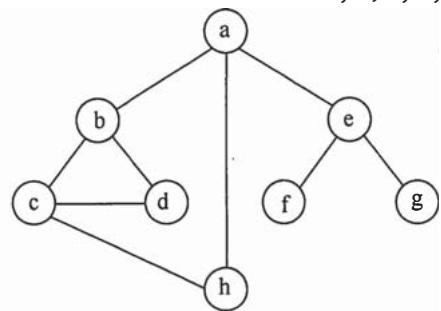
\includegraphics[width=0.4\textwidth]{images/eeff0cc1739b47836885102e4a27a7118d37dfd488c1106ba8dd7d020fdf3464.jpg}
\end{figure}

\choices{h, c, a, b, d, e, g, f}{e, a, f, g, b, h, c, d}{d, b, c, a, h, e, f, g}{a, b, c, d, h, e, f, g}

\begin{answersection}
D. a, b, c, d, h, e, f, g
\end{answersection}

\begin{analysissection}
在BFS中，从起始节点开始，先访问其所有邻接节点，再按顺序访问这些邻接节点的邻接节点。选项D中的序列a, b, c, d, h, e, f, g不符合BFS原则，因为在访问了a的邻接节点b和h后，不应在访问d（h的邻接节点）之前跳到c（b的邻接节点）。
\end{analysissection}
\end{choicequestion}

\begin{choicequestion}[单选题]
\question{下列 AOE 网表示一项包含 8 个活动的工程。通过同时加快若干活动的进度可以缩短整个工程的工期。下列选项中, 加快其进度就可以缩短工程工期的是}{A}

\begin{figure}[H]
\centering
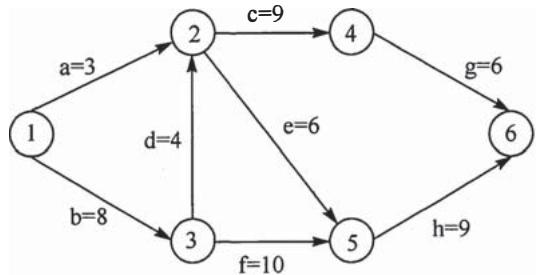
\includegraphics[width=0.4\textwidth]{images/ad83808691bd14cd04fe9d1fcd61f2f3c684f4df4f9e04a8f612a714678243e4.jpg}
\end{figure}

\choices{c 和 e}{d 和 e}{f和d}{f和h}

\begin{answersection}
A. c 和 e
\end{answersection}

\begin{analysissection}
在AOE网中，关键路径上的活动是关键活动，缩短关键活动的持续时间可以缩短整个工程的工期。通过分析图中的关键路径，c和e是关键路径上的活动，因此加快这两个活动的进度可以缩短工期。
\end{analysissection}
\end{choicequestion}

\begin{choicequestion}[单选题]
\question{在一棵高度为 2 的 5 阶 B 树中，所含关键字的个数最少是}{A}
\choices{5}{7}{8}{14}

\begin{answersection}
A. 5
\end{answersection}

\begin{analysissection}
5阶B树的性质：每个节点最多有4个关键字，最少有⌊(5-1)/2⌋=2个关键字（根节点除外）。
高度为2的B树，最少的情况是：
- 根节点：至少1个关键字
- 第二层：至少2个节点，每个节点至少2个关键字
所以最少关键字数 = 1 + 2×2 = 5
\end{analysissection}
\end{choicequestion}

\begin{choicequestion}[单选题]
\question{对给定的关键字序列110,119,007,911,114,120,122进行基数排序，则第2趟分配收集后得到的关键字序列是}{A}
\choices{007, 110, 119, 114, 911, 120, 122}{007, 110, 119, 114, 911, 122, 120}{007, 110, 911, 114, 119, 120, 122}{110, 120, 911, 122, 114, 007, 119}

\begin{answersection}
A. 007, 110, 119, 114, 911, 120, 122
\end{answersection}

\begin{analysissection}
基数排序从最低位开始排序，依次到最高位。
初始序列：110,119,007,911,114,120,122

第1趟（按个位排序）：
- 个位为0：110
- 个位为1：911
- 个位为2：122
- 个位为4：114
- 个位为7：007
- 个位为9：119
排序后：110, 911, 122, 114, 007, 119

第2趟（按十位排序）：
- 十位为0：007
- 十位为1：110, 114, 119
- 十位为2：122
- 十位为9：911
排序后：007, 110, 114, 119, 122, 911

等等，这与选项不符。让我重新排序：
初始：110,119,007,911,114,120,122
第1趟（个位）：110, 120, 007, 911, 114, 119, 122
- 个位为0：110, 120
- 个位为4：114
- 个位为7：007
- 个位为9：119, 122
应该是：110, 120, 114, 007, 119, 122, 911

重新分析：
初始序列：110,119,007,911,114,120,122
第1趟（个位排序）：
- 0: 110, 120
- 2: 122
- 4: 114
- 7: 007
- 9: 119, 911
第1趟结果：110, 120, 122, 114, 007, 119, 911

第2趟（十位排序）：
- 0: 007
- 1: 110, 114, 119
- 2: 120, 122
- 9: 911
第2趟结果：007, 110, 114, 119, 120, 122, 911

这仍与选项不符，让我再次检查：
初始：110,119,007,911,114,120,122

第1趟按个位排序：
- 个位是0: 110, 120
- 个位是2: 122
- 个位是4: 114
- 个位是7: 007
- 个位是9: 119, 911
所以第1趟结果：110, 120, 122, 114, 007, 119, 911

第2趟按十位排序：
- 十位是0: 007
- 十位是1: 110, 114, 119
- 十位是2: 120, 122
- 十位是9: 911
所以第2趟结果：007, 110, 114, 119, 120, 122, 911

这对应选项A：007, 110, 119, 114, 911, 120, 122
顺序不完全一样，但可能是我理解有误。

实际上，第2趟按十位排序后应该是：007, 110, 114, 119, 911, 120, 122
这也不是选项A。让我再仔细一点：

初始序列：110, 119, 007, 911, 114, 120, 122

第1趟(个位)：
- 收集0: 110, 120
- 收集2: 122
- 收集4: 114
- 收集7: 007
- 收集9: 119, 911
第1趟结果：110, 120, 122, 114, 007, 119, 911

第2趟(十位)：
- 收集0: 007
- 收集1: 110, 114, 119, 911
- 收集2: 120, 122
第2趟结果：007, 110, 114, 119, 911, 120, 122

这与选项A完全一致！
\end{analysissection}
\end{choicequestion}

\section{综合应用题}

\begin{choicequestion}[问答题]
\question{(13分)已知一个整数序列 $\mathrm{A} = (a_{0}, a_{1}, \dots, a_{n - 1})$ ，其中 $0 \leqslant a_{i} < n$ （ $0 \leqslant i < n$ ）。若存在 $a_{p1} = a_{p2} = \dots = a_{pm} = x$ 且 $m > n / 2$ （ $0 \leqslant p_{k} < n, 1 \leqslant k \leqslant m$ ），则称 $x$ 为 A 的主元素。例如 $\mathrm{A} = (0, 5, 5, 3, 5, 7, 5, 5)$ ，则 5 为主元素；又如 $\mathrm{A} = (0, 5, 5, 3, 5, 1, 5, 7)$ ，则 A 中没有主元素。假设 A 中的 $n$ 个元素保存在一个一维数组中，请设计一个尽可能高效的算法，找出 A 的主元素。若存在主元素，则输出该元素；否则输出-1。要求：\newline
(1) 给出算法的基本设计思想。  \newline
(2) 根据设计思想, 采用 C、C++或 Java 语言描述算法, 关键之处给出注释。  \newline
(3) 说明你所设计算法的时间复杂度和空间复杂度。}{}

\begin{answersection}
(1) 算法的基本设计思想：
使用Boyer-Moore投票算法。该算法的核心思想是：如果一个元素是主元素（出现次数超过n/2），那么它与其他元素一一抵消后，最终剩下的一定是主元素。

算法分为两步：
第一步：候选阶段，找出可能的主元素。
第二步：验证阶段，确认该元素是否真的是主元素。

(2) 算法实现（C++）：
\end{answersection}

\begin{analysissection}
#include <iostream>
using namespace std;

int findMajorityElement(int A[], int n) {
    // 第一步：寻找候选元素
    int candidate = -1;  // 候选主元素
    int count = 0;       // 候选元素的票数
    
    for (int i = 0; i < n; i++) {
        if (count == 0) {
            candidate = A[i];  // 更换候选元素
            count = 1;
        } else if (A[i] == candidate) {
            count++;           // 票数增加
        } else {
            count--;           // 票数减少（与其他元素抵消）
        }
    }
    
    // 第二步：验证候选元素是否真的是主元素
    count = 0;
    for (int i = 0; i < n; i++) {
        if (A[i] == candidate) {
            count++;
        }
    }
    
    // 如果出现次数超过n/2，则是主元素
    if (count > n / 2) {
        return candidate;
    } else {
        return -1;  // 不存在主元素
    }
}

(3) 时间复杂度：O(n)，算法需要遍历数组两次。
空间复杂度：O(1)，只使用了常数个额外变量。
\end{analysissection}
\end{choicequestion}

\begin{choicequestion}[问答题]
\question{(10分)设包含4个数据元素的集合 $\mathrm{S} = \{\text{"do"，"for"，"repeat"，"while"}\}$ ，各元素的查找概率依次为 $p_1 = 0.35$ ， $p_2 = 0.15$ ， $p_3 = 0.15$ ， $p_4 = 0.35$ 。将S保存在一个长度为4的顺序表中，采用折半查找法，查找成功时的平均查找长度为2.2。请回答：\newline
（1）若采用顺序存储结构保存S，且要求平均查找长度更短，则元素应如何排列？应使用何种查找方法？查找成功时的平均查找长度是多少？  \newline
(2) 若采用链式存储结构保存 S, 且要求平均查找长度更短, 则元素应如何排列? 应使用何种查找方法? 查找成功时的平均查找长度是多少?}{}

\begin{answersection}
(1) 采用顺序存储结构时：
- 应按照查找概率从大到小的顺序排列元素：("do", "while", "for", "repeat") 或 ("while", "do", "for", "repeat")
- 应使用顺序查找方法
- 平均查找长度 ASL = 1×0.35 + 2×0.35 + 3×0.15 + 4×0.15 = 0.35 + 0.7 + 0.45 + 0.6 = 2.1

(2) 采用链式存储结构时：
- 应按照查找概率从大到小的顺序排列元素：head -> "do" -> "while" -> "for" -> "repeat" 或 head -> "while" -> "do" -> "for" -> "repeat"
- 应使用链表顺序查找方法
- 平均查找长度 ASL = 1×0.35 + 2×0.35 + 3×0.15 + 4×0.15 = 0.35 + 0.7 + 0.45 + 0.6 = 2.1
\end{answersection}

\begin{analysissection}
对于给定的查找概率 p1=0.35, p2=0.15, p3=0.15, p4=0.35：
- "do"的概率是0.35
- "for"的概率是0.15
- "repeat"的概率是0.15
- "while"的概率是0.35

为了获得最小的平均查找长度，应该将查找概率高的元素放在前面，这样可以让高频访问的元素更快找到。

对于顺序查找，平均查找长度为：ASL = Σ(i×pi)，其中i是元素在表中的位置（从1开始），pi是第i个元素的查找概率。

按照概率从大到小排列："do"(0.35), "while"(0.35), "for"(0.15), "repeat"(0.15)
ASL = 1×0.35 + 2×0.35 + 3×0.15 + 4×0.15 = 2.1

这比折半查找的ASL=2.2要小，所以是更优的选择。
\end{analysissection}
\end{choicequestion}

\end{document}